\chapter{Technol\'ogia}\label{chapter:technologia}
\section{Felhasználói felület}
Az alkalmazás felhasználói felületét a React \cite[]{react} könyvtár segítségével valósítottam meg.
A React egy nyílt forráskódú JavaScript könyvtár, amelyet a Facebook fejlesztett ki.
A könyvtár célja, hogy a felhasználói felület fejlesztését egyszerűbbé tegye.
A React egy komponens alapú könyvtár, amely lehetővé teszi a fejlesztők számára,
hogy újra felhasználható komponenseket hozzanak létre, amelyeket összeállítva
komplex felhasználói felületeket hozhatnak létre.
\\
\\
\textbf{Komponensek}
A React komponensek egyfajta sablonok, amelyek a felhasználói felület egy részét írják le.
A komponensek egy egyszerű JavaScript objektumok, amelyeknek van egy render metódusa,
amely visszaadja a komponens felhasználói felületét.
\\
\\
\textbf{Komponensek főbb tulajdonságai:}
\begin{itemize}
    \item Paraméterek (props)
    \item Gyerekei (children)
    \item Állapotai (state)
    \item Életciklus metódusai (lifecycle)
    \item Eseménykezelői (event)
    \item Stílusai (style)
    \item Referenciák (ref)
    \item Kontextusai (context)
    \item Típusai (type)
    \item Kulcsai (key)
\end{itemize}
\subsection{React és Angular összehasonlítása}
React\cite[]{react} és Angular\cite[]{angular} két népszerű front-end fejlesztési eszköz, amelyek a modern webalkalmazások építésének alapkövei. Mindkettő előnyöket és hátrányokat kínál a webfejlesztés különböző aspektusaiban.
\subsection*{Könyvtár vs. Keretrendszer}
\begin{itemize}
  \item React egy felhasználói felület-építő könyvtár, míg Angular egy teljeskörű MVC keretrendszer.
\end{itemize}
\subsection*{Adatkötés}
\begin{itemize}
  \item React támogatja az egyirányú adatkötést, ami elősegíti a hibakeresést.
  \item Angular kétféle adatkötést kínál: egyirányú és kétirányú, ami megkönnyíti a fejlesztést, de bonyolultabb alkalmazásoknál teljesítménybeli költségekkel járhat.
\end{itemize}
\subsection*{Teljesítmény}
\begin{itemize}
  \item React-ben a virtuális DOM használata javítja a teljesítményt, különösen dinamikus tartalom esetén.
  \item Angular-ban a kétirányú adatkötés növelheti a teljesítményigényt nagy adatkészletek esetén.
\end{itemize}
\subsection*{Tanulási Görbe}
\begin{itemize}
  \item React viszonylag egyszerű megérteni, különösen azok számára, akik már ismerik a JavaScriptet.
  \item Angular magasabb tanulási görbével rendelkezik az összetett szintaxis és a keretrendszer által kínált széleskörű funkciók miatt.
\end{itemize}
\subsection*{Közösség és Ökoszisztéma}
\begin{itemize}
  \item Mind React, mind Angular rendelkezik egy nagy és aktív közösséggel, bár eltérő előnyökkel és kihívásokkal.
\end{itemize}

\subsection{Redux vagy Context API}
Az alkalmazás állapotainak kezelésére több lehetőség is felmerült, közöttük a Redux és a Context API.
A Redux \cite[]{redux} egy állapotkezelő könyvtár, amely lehetővé teszi az alkalmazás állapotának tárolását egy központi helyen.
A Context API egy React API, amely lehetővé teszi az alkalmazás állapotának tárolását és megosztását a komponensek között.
Mivel az alkalmazás kis méretű, ezért a Context API-ra esett a választás.
\\
\\
\textbf{A Context API főbb tulajdonságai:}
\begin{itemize}
    \item \textbf{Beépített megoldás:} A Context API része a React alapkönyvtárnak, nincs szükség külső függőségekre.
    \item \textbf{Egyszerűség:} A Context API egyszerűbb és könnyen megérthető, kevesebb boilerplate kóddal.
    \item \textbf{Nincs middleware:} Nem támogat middleware-eket alapból, így aszinkron állapotfrissítéseket manuálisan kell kezelni.
    \item \textbf{Nem optimalizált nagy alkalmazásokhoz:} Nagy alkalmazásokban hatékonytalan lehet, mert minden Context változásra újrarendereli az összes fogyasztót, hacsak nem optimalizáljuk manuálisan.
    \item \textbf{Kevesebb eszköz:} Kevesebb beépített eszköze van, mint a Redux-nak, de ez nem mindig hátrány, függ a projekt igényeitől.
\end{itemize}

\textbf{A Redux főbb tulajdonságai:}
\begin{itemize}
    \item \textbf{Optimalizáció:} Redux kifejezetten optimalizált a nagyobb alkalmazások számára, és lehetővé teszi az állapot frissítéseinek finom szabályozását.
    \item \textbf{Middleware Támogatás:} Redux lehetőséget ad middleware-ek használatára, amelyek lehetővé teszik az aszinkron állapotfrissítések könnyebb kezelését.
    \item \textbf{Tesztelhetőség:} A Redux architektúrája miatt a tesztelés egyszerűbb, minden action egy független egység, és a reducer funkciók tiszta függvények.
    \item \textbf{Eszközök és Közösség:} Redux-nak nagy közössége van, és sok kiegészítő eszköz, például a Redux DevTools.
    \item \textbf{Boilerplate Kód:} Több boilerplate kód szükséges, hogy elindítsunk egy Redux-alapú állapotkezelést.
\end{itemize}

\subsection{TypeScript vagy JavaScript}
A TypeScript egy nyílt forráskódú, szigorúan típusos programozási nyelv,
amely a JavaScriptre épül, lehetővé teszi a statikus típusok használatát,
és minden érvényes JavaScript kód érvényes TypeScript kódnak is számít.
Inkább a TypeScript mellett döntöttem, mert a statikus típusok használata
növeli a kód minőségét és a fejlesztési sebességet, illetve csökkenti a hiba lehetőségek számát.

\section{Szerveroldali Logika és API-k}
A szerver és a kliens közötti kommunikáció megvalósításához az ASP.NET Core-t használtam.
Az ASP.NET Core egy nyílt forráskódú, cross-platform, magas teljesítményű keretrendszer,
amelyet a Microsoft fejlesztett ki.
Az ASP.NET Core-t a webalkalmazások és a webes API-k fejlesztésére használják.
A környezetet a C\# programozási nyelvhez tervezték, de támogatja a többi .NET nyelvet is.
Én a megvalósítás során a C\# nyelvet használtam.
Ebben a fejezetben bemutatom a szerveroldali logikát és az API-kat.

\subsection{Adatbázis}
Az alkalmazásnál MS SQL adatbázist használtam, mert a Microsoft SQL Server-t használom a személyes projekteimhez.
Az MS SQL (Microsoft SQL Server) egy relációs adatbázis-kezelő rendszer (RDBMS) a Microsofttól. Jól skálázható, és számos fejlett funkcióval rendelkezik,
mint például tárolt eljárások,
triggerek és nézetek
. Gyakran használják vállalati szintű alkalmazásokban,
és támogatja a SQL nyelvet az adatok lekérdezésére és manipulálására.
Támogatja az ACID tulajdonságokat és a tranzakciós integritást.
Az ER modell-t használtam az adatbázis tervezéséhez.
Ezt majd a Backend fejlesztési folyamatánál részletezem.

\subsection{Entity Framework Core}
Az Entity Framework Core \cite[]{efcore} (EF Core) egy objektum-relációs leképzési (ORM) keretrendszer a Microsofttól,
amely .NET Core és .NET 5+ alkalmazások számára készült.
Lehetővé teszi a fejlesztők számára, hogy magas szintű,
objektumorientált API-n keresztül dolgozzanak adatbázisokkal,
anélkül hogy közvetlen SQL lekérdezéseket kellene írniuk.
Támogatja a code-first és a database-first megközelítéseket,
így rugalmasságot biztosít az adatmodell és az adatbázisséma kialakításában. Az EF Core lehetővé teszi a LINQ (Language Integrated Query) használatát,
ami természetes módon illeszkedik a C\# és más .NET nyelvekhez.

\begin{figure}[H]
    \centering
    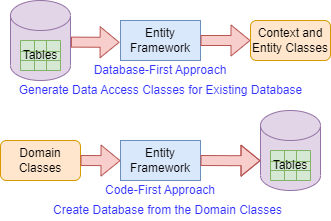
\includegraphics[width=14.0truecm]{images/EntityFramework.png}
    \caption{Entity Framework Core}
    \label{fig:entity_framework_core}
\end{figure}

Skálázható és teljesítmény-optimalizált, ezért alkalmas mind kis,
mind nagyobb vállalati projektekben. Az EF Core támogatja a többszörös adatbázis-motorokat, beleértve az SQL Server-t, PostgreSQL-t, SQLite-ot és másokat is.
Az adatmigrációk egyszerű kezelése és automatikus generálása az egyik előnye, ami könnyebbé teszi az adatbázis séma változásainak kezelését.
A keretrendszer beépített támogatással rendelkezik a tranzakciókezelésre, így az ACID tulajdonságok biztosítottak. Az EF Core rugalmas konfigurációs lehetőségekkel rendelkezik,
és jól integrálódik más .NET Core szolgáltatásokkal, mint például a Dependency Injection. Folyamatosan fejlődik és aktívan karbantartott,
így a legújabb .NET technológiákhoz és az adatbázis-technológiákhoz is gyorsan alkalmazkodik.

\subsection{API}
A komponensek közötti kommunikáció megvalósítására RESTful API-t használtam, annak népszerűsége miatt. A REST (Representational State Transfer) egy architektúrális stílus,
amelyet a webes alkalmazásokhoz használnak. A RESTful API-kat a REST architektúra alapelvei alapján tervezik.
A RESTful API-kat a HTTP protokollra építik, és a HTTP metódusokat használják a kérések kezelésére.
Ennek megvalósításához a \textit{ControllerBase} osztályt használtam a Controllerekben.
Ami teljesen implementálja a RESTful API-kat, és a HTTP metódusokat.

\begin{figure}[H]
    \centering
    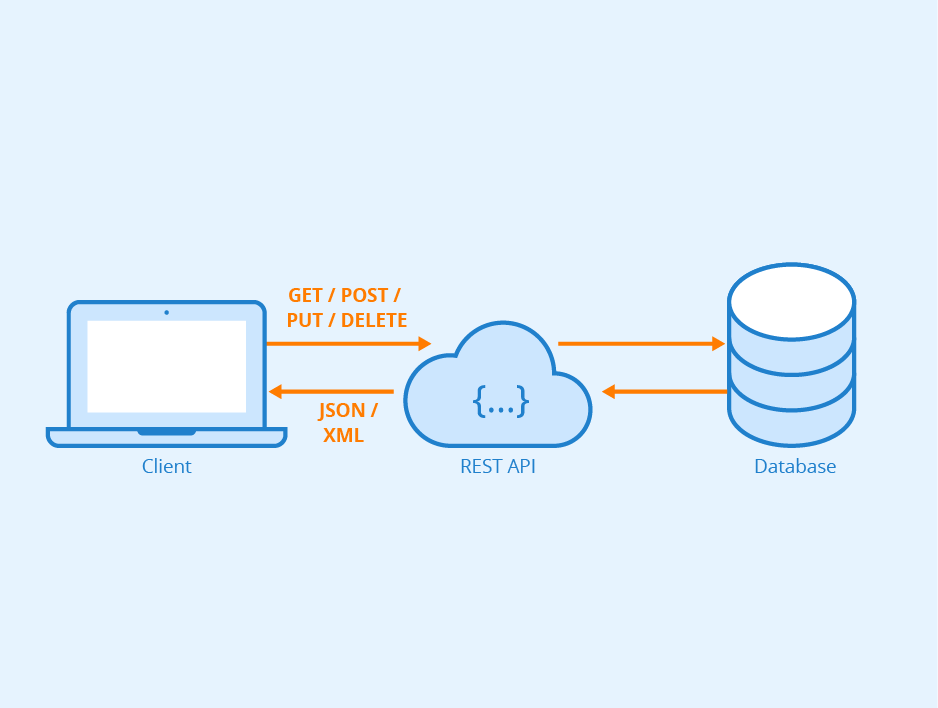
\includegraphics[width=14.0truecm]{images/Rest-API.png}
    \caption[RESTful API]{RESTful API \cite{restfulapi}}
    \label{fig:restfulapi}
\end{figure}

A videók lejátszása során különös figyelmet fordítottam
az állapotkezelésre. Ennek érdekében a WebSocket
protokollt alkalmaztam. A WebSocket egy kétirányú
kapcsolatot tesz lehetővé a böngésző és a szerver között.
Bár a HTTP protokollra épül, mégis képes valós idejű
kommunikációra. A kommunikáció HTTP portokon keresztül zajlik,
ami rugalmasságot ad az alkalmazásnak.
SignalR-t használtam a WebSocket protokoll megvalósításához.

A SignalR egy Microsoft által fejlesztett aszinkron könyvtár,
amely valós idejű webes alkalmazások építését támogatja.
Lehetővé teszi a szerver és a kliensek közötti kétirányú
kommunikációt, gyakran WebSockets használatával.

\begin{figure}[H]
    \centering
    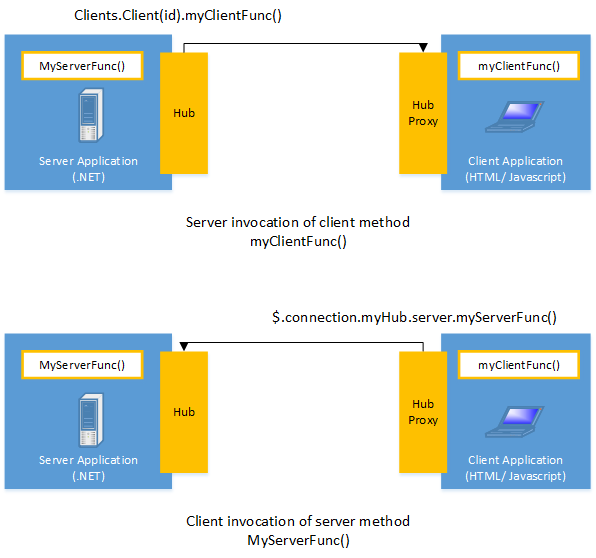
\includegraphics[width=14.0truecm]{images/SignalR.png}
    \caption[SignalR]{SignalR \cite{signalR}}
    \label{fig:signalR}
\end{figure}
Ez eltér a hagyományos HTTP modelltől,mivel a szerver aktívan küldhet üzeneteket a klienseknek.
Gyakori alkalmazási területei közé tartoznak a chat szolgáltatások,
online játékok és élő adatfrissítések. A SignalR automatikusan választja ki a legmegfelelőbb kommunikációs mechanizmust a szerver és a kliens között,
például long polling, ha WebSockets nem érhető el. A könyvtár könnyen integrálható más .NET technológiákkal és keretrendszerekkel, például ASP.NET Core-al.
A SignalR segítségével könnyen implementálhatók komplex forgatókönyvek, például csoportos üzenetküldés vagy kapcsolatok kezelése. Az állapotkezelés és a kiváló skálázhatóság további előnyei a SignalR használatának.
Mivel a SignalR API az ASP.NET Core része, az infrastruktúrát és a biztonsági mechanizmusokat is könnyen ki lehet terjeszteni rá. Összességében a SignalR egy erőteljes eszköz a valós idejű webes alkalmazások fejlesztéséhez.

\subsection{Fejlesztői környezet}
Én a Visual Studio 2022-t \cite[]{vsstudio} használtam a fejlesztéshez, mert ez az egyik legnépszerűbb IDE a .NET fejlesztők körében.
A Visual Studio 2022 egy integrált fejlesztői környezet (Integrated Development Environment, IDE), amelyet a Microsoft fejlesztett ki. Ez a platform különösen népszerű a Windows alapú alkalmazások fejlesztésénél, de támogatja számos programozási nyelvet és technológiát, így a fejlesztők széles spektruma számára kínál megoldásokat. Az IDE magába foglalja a kódszerkesztést, a debuggolást, a verziókezelést és más, a fejlesztési ciklusban fontos eszközöket is.

\begin{figure}[H]
    \centering
    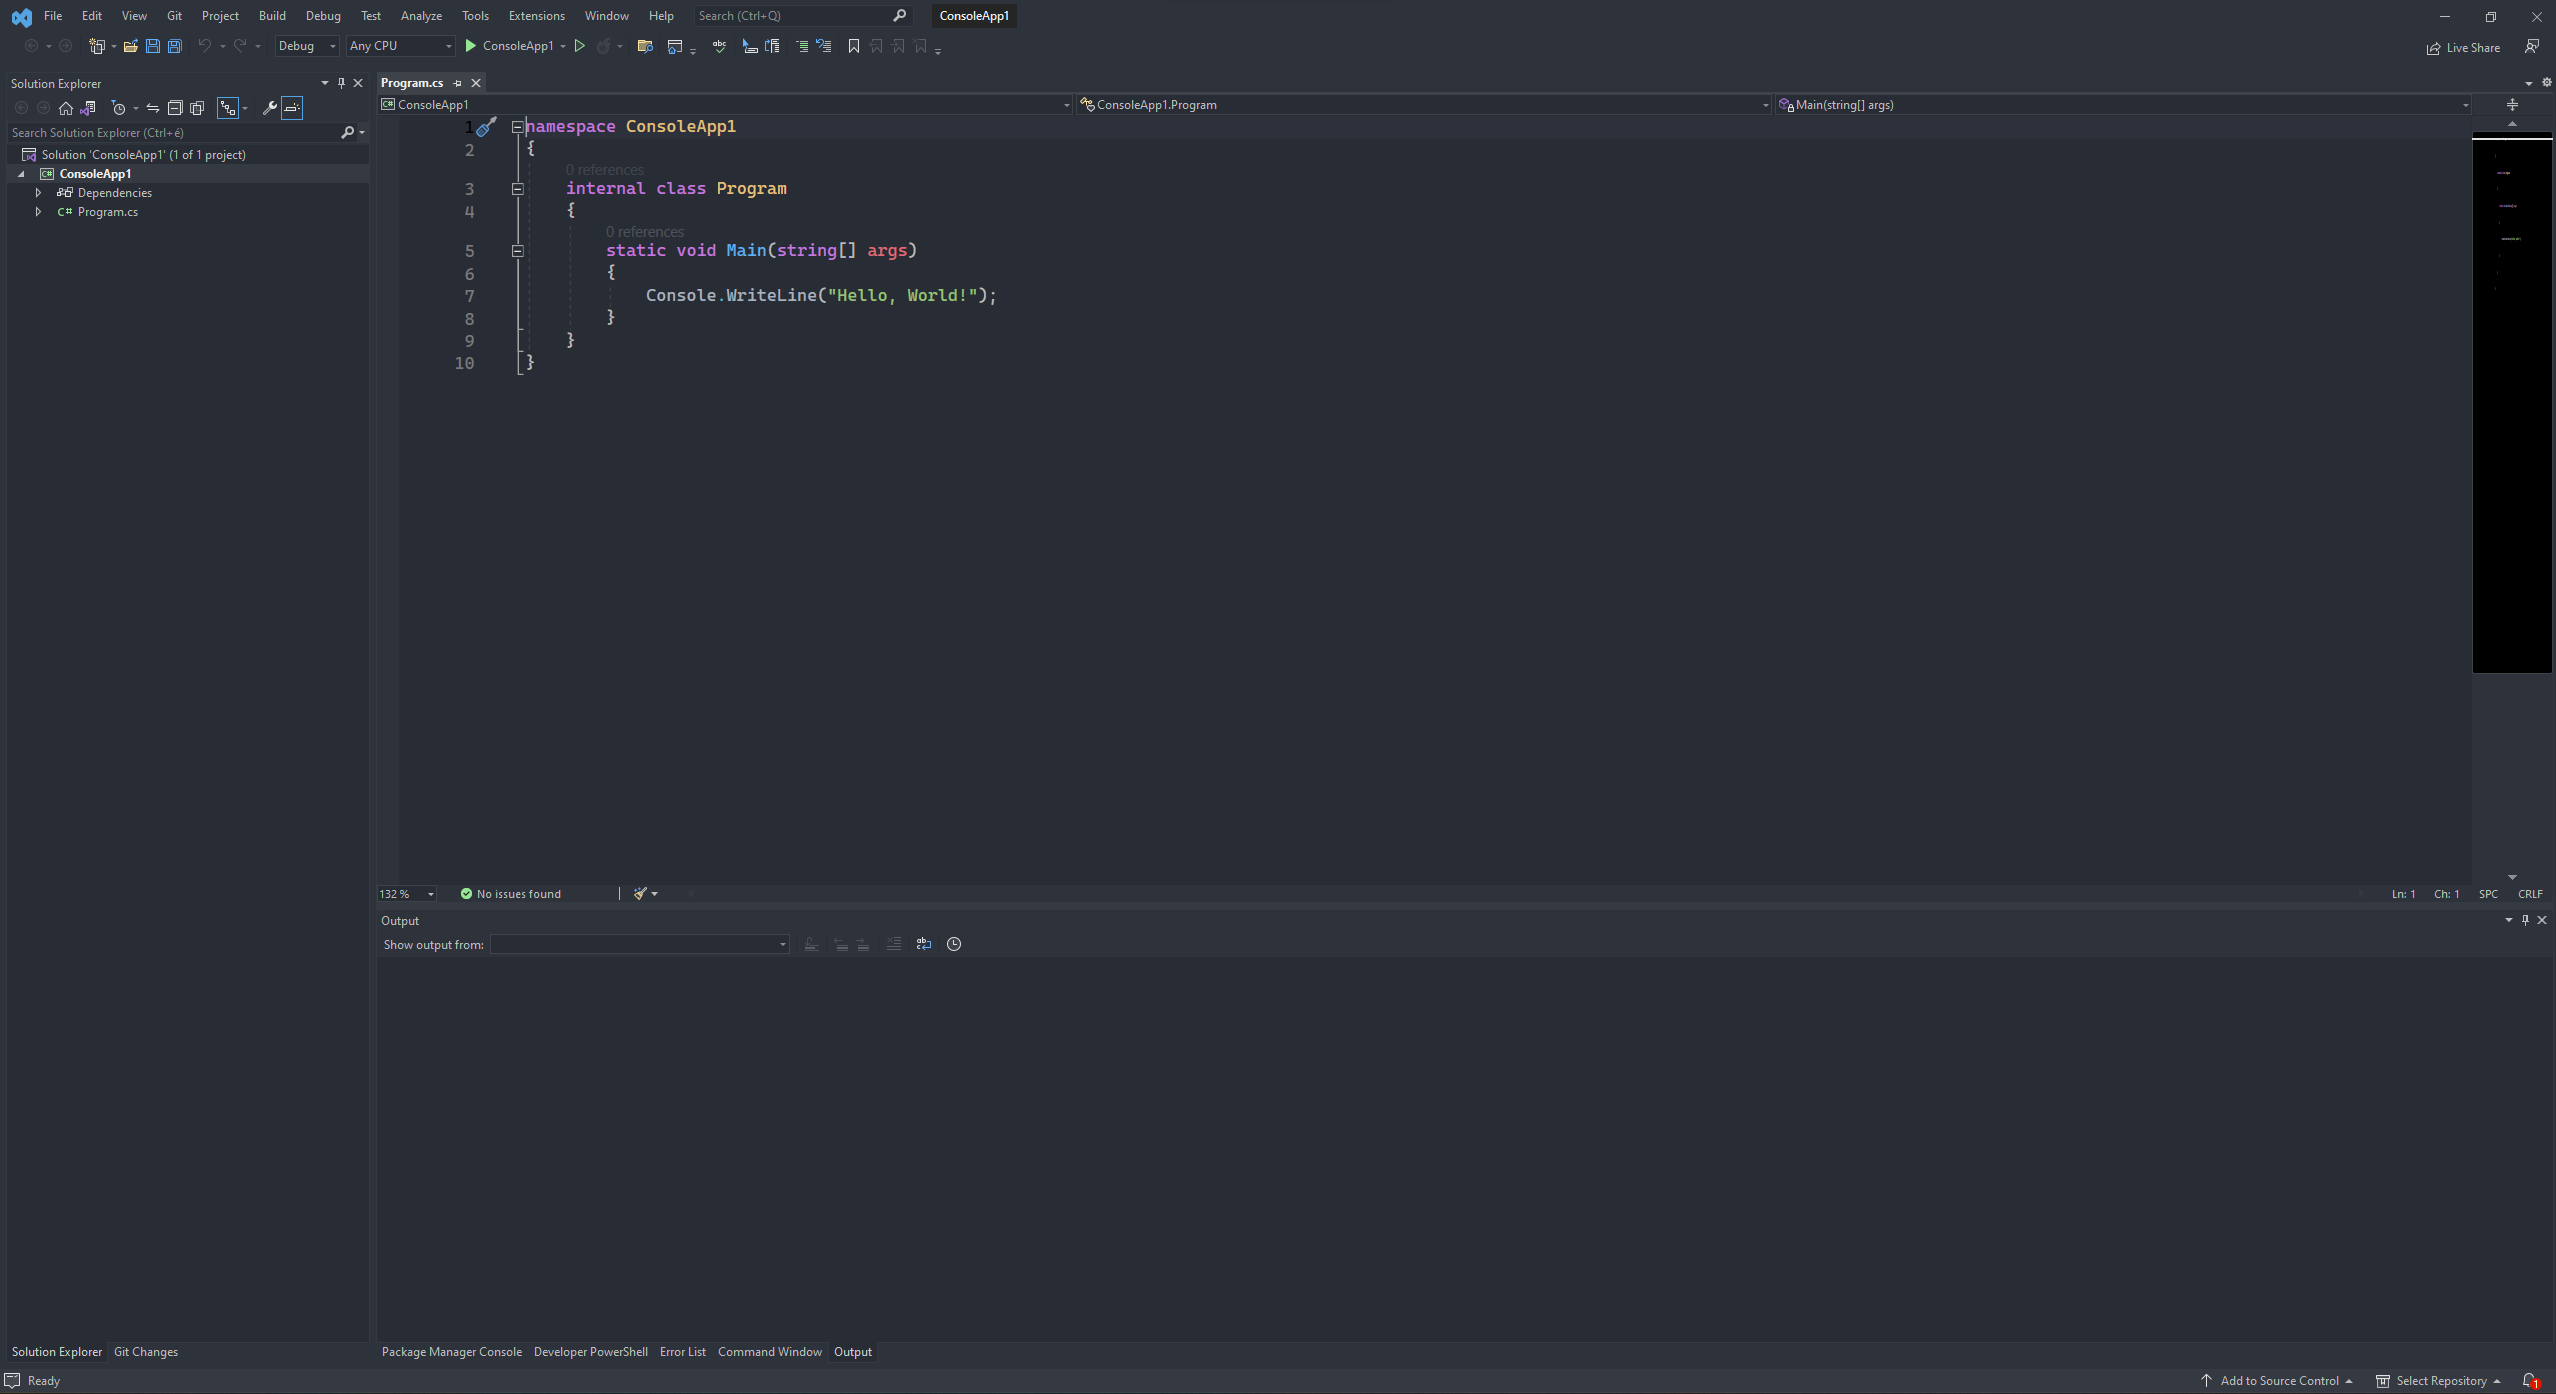
\includegraphics[width=14.0truecm]{images/VisualStuido2022.png}
    \caption{Visual Studio 2022}
    \label{fig:VisualStuido2022}
\end{figure}
Míg a Visual Studio elsősorban a Windows operációs rendszerre lett tervezve, a Microsoft kiadott egy könnyebb, keresztplatformos változatot is, a Visual Studio Code-ot. Ez utóbbi támogatja a Linux és macOS operációs rendszereket is, így a fejlesztők választhatnak az operációs rendszerüknek legmegfelelőbb változat közül.

Mindkét platform lehetővé teszi az együttműködést és a csapatmunkát, és számos bővítményt és sablont kínál a gyors és hatékony fejlesztés érdekében.
\section{Publikálással kapcsolatos eszközök}
\subsection{Docker}
Docker egy nyílt forráskódú konténerizációs technológia, amely lehetővé teszi az alkalmazások csomagolását és izolált környezetben való futtatását, biztosítva ezzel az alkalmazások környezettől független működését. Ennek köszönhetően a Docker kulcsfontosságú eszköz a fejlesztési és üzemeltetési folyamatok egyszerűsítésében.
\\
\textbf{Docker használatának előnyei:}
\begin{itemize}
  \item \textbf{Környezeti konzisztencia:} Ugyanazt a környezetet biztosítja fejlesztési, tesztelési és termelési fázisokban, csökkentve a kompatibilitási problémákat.
  \item \textbf{Gyors telepítés:} Konténerek segítségével az alkalmazások gyorsan telepíthetők és indíthatók, növelve a fejlesztési ciklus hatékonyságát.
  \item \textbf{Skálázhatóság:} Egyszerűen kezelhető az alkalmazások skálázása konténerek hozzáadásával vagy eltávolításával.
  \item \textbf{Izoláció:} Az alkalmazások egymástól függetlenül futnak, növelve ezzel a rendszer biztonságát és stabilitását.
  \item \textbf{Egyszerű karbantartás:} A Docker képek frissítése és a konténerek újraindítása egyszerűen kezelhető, csökkentve a szolgáltatáskimaradásokat.
  \item \textbf{Könnyű konfiguráció:} A konfigurációk és függőségek egy konténerbe csomagolhatók, így azok könnyen átvihetők különböző környezetek között.
\end{itemize}
\begin{figure}[H]
    \centering
    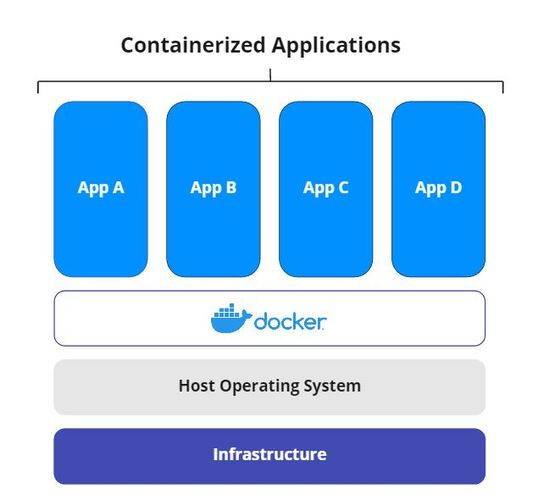
\includegraphics[width=14.0truecm]{images/docker.jpg}
    \caption{Docker\cite[]{docker} arhitektúra}
    \label{fig:docker}
\end{figure}
\subsection{Drone CI}
Drone CI egy nyílt forráskódú, konténer-alapú folyamatos integrációs és folyamatos kiszállítási (CI/CD) platform, amely automatizálja a szoftverfejlesztési folyamatokat, mint például a kódépítést, tesztelést és telepítést. A Drone legfontosabb jellemzői közé tartozik a könnyű konfigurálhatóság, a magas szintű skálázhatóság és a konténerizáció által nyújtott izoláció.
\\
\textbf{Drone CI használatának előnyei:}
\begin{itemize}
  \item \textbf{Könnyű Konfigurálhatóság:} A Drone a \texttt{.drone.yml} konfigurációs fájlt használja, amelyet a projekt gyökérkönyvtárában helyeznek el, így egyszerűvé téve a CI/CD folyamatok meghatározását és konfigurálását.
  \item \textbf{Konténer-alapú Izoláció:} Minden feladat Docker konténerekben fut, biztosítva a környezeti konzisztenciát és az izolációt a folyamatok között.
  \item \textbf{Plug-in Rendszer:} A Drone széles körű plug-in támogatással rendelkezik, amely lehetővé teszi külső szolgáltatások, mint például adatbázisok, értesítési rendszerek és telepítési eszközök integrálását.
  \item \textbf{Automatizált Tesztelés és Telepítés:} A Drone automatizálja a kódépítést, a tesztek futtatását és az alkalmazások különböző környezetekbe való telepítését, így javítva a fejlesztési ciklus sebességét és hatékonyságát.
  \item \textbf{Skálázhatóság:} A Drone architektúrája lehetővé teszi a könnyű skálázást, akár nagyobb terhelés mellett is, biztosítva a gyors és hatékony CI/CD folyamatokat.
\end{itemize}